\chapter{State of the Art\label{cha:chapter2}}
This chapter introduces the necessary background knowledge to follow the concept and implementation of this thesis. OD illuminates an abstract approach of pose detection and how image processing is currently present in manufacturing. Furthermore, important aspect of SOAs will be introduced, especially service interfaces, semantics and deployment options. Lastly, OPC UA Vision as a provider for an information model and a state machine for vision systems illustrates the current efforts in vendor interoperability in machine vision.

\section{Object Detection}
OD is a computer technology for identifying instances of objects in digital images or videos~\cite{Hornberg2017HandbookVision}. As one of the goals of this thesis is to empower manufacturers to exchange object detection methods (ODM) quickly, there are two aspects which need to be considered. First, the current state of OD in manufacturing should be summarized for an understanding of what the proposed framework has to cope with. Second, contemporary object detectors should be reviewed to find a least common denominator for an interface.

\subsection{Image Processing in Manufacturing}
Image processing tasks in manufactoring are categorized into evaluations such as inspection, monitoring, verification and recognition~\cite{Hornberg2017HandbookVision}. For a long time, image processing systems were used to identify bad or incomplete parts which were then scrapped. The systems were not used for complex tasks and the result of the process was usually boolean. With progress in OD, value adding processes have enhanced image processing tasks. For example, robots can be guided with depth cameras or a welding process can be not only monitored but also looped back and controlled. OD serves as the eyes and - to some extent - the brain for the robot. Challenges in OD such as bin picking can now be tackled. 

Furthermore, integration of an image processing system in manufacturing (and other domains) is a highly specific task. Usually, a machine vision expert has to program and configure the system for every new machine type or even every machine. Small companies cannot afford such experts~\cite{Hornberg2017HandbookVision}. They are capable of maintaining the system and other repetitious tasks when the documentation is suitable. Subsequently, system integrators tend to offer rigid turn-key-solutions with a specific user interface. On the inside, the frameworks that system integrators sell are made of reusable applications~\cite{Hornberg2017HandbookVision}.

\subsection{Two Phases of Object Detection}
Coming from a world of mostly black and white 2D images, OD research has recently advanced to colored depth 3D images through rising computing power~\cite{Hornberg2017HandbookVision}. With the added dimension, it is possible to determine the pose of an object in a camera image. Pose detection can be split into two parts: a 3D model of an object serves as training input to generate necessary features or templates (phase 1).  After training, the object can be detected in RGB-D images with the help of the training output (phase 2). 

Phase 1 is a routine that is necessary for successful pose detection. More than a thousand templates can be generated in this phase. Without the use of automation, the cost/benefit calculation of this phase would never call for using OD. Every template including the angle from which it was acquired would have to be measured and mapped to the template. Subsequently, in recent algorithms, CAD files were used for this purpose. 

An example method of phase 2 is template matching (TM). Fig.~\ref{templatematching} illustrates the process. In the left image, the face of the man is to be found. The template is the little cut-out in the middle. Pixel by pixel, the template is being convoluted with the original image and rated with a metric. The resulting resolution matrix is depicted on the right. Bright areas indicate potential findings. At the brightest point, the template is rightfully suggested.~\cite{OpenCV-Documentation2018Template2018}

\begin{figure}[ht]
	\centering
  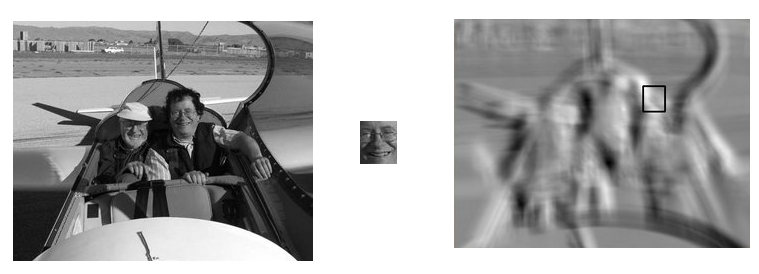
\includegraphics[width=\textwidth]{templatematching.png}
	\caption[Template Matching]{In the picture on the left, the template in the middle is to be found. Depicted on the right is the resolution matrix with potential findings indicated with the bright color and the found area of the template in the original image.~\cite{OpenCV-Documentation2018Template2018}}
	\label{templatematching}
\end{figure}

Especially in the last decade, 6D pose estimation gained popularity (\cite{Drost2010ModelRecognition}, \cite{Sundermeyer2018ImplicitImages} \cite{Hinterstoisser2013ModelScenes}). In 2018, Hodaň benchmarked 15 ODMs which share the approach of two-phased pose detection~\cite{Hodan2018BOP:Estimation}. He categorized the methods in template, point-pair-feature, local-feature and learning-based. His evaluation showed that point-pair-feature-based methods currently perform best measured against a pose-error function that deals with pose ambiguities.

To summarize, pose detection is generally split into a preparation and a detection phase. When designing a framework dealing with quickly changing ODMs, this ODM-agnostic process description should be taken into account.

\section{Service-Oriented Architectures}
SOA is a software design paradigm which gained importance towards monolithic approaches. Its main advantages over monolithic approaches are scalability, decoupling of components and simple development, testing and deployment~\cite{Richards2015MicroservicesArchitecture}. Services are concise, decoupled components capable of one specific task~\cite{Newman2015BuildingMicroservices}. The goal is to design services for maximum reusability. Together, either orchestrasted or choreographing, they form an application.

The following subsections focus on how services can be interfaced and deployed.

\subsection {Service Interfaces}
\label{serviceinterfaces}
In this section, potential client-server-based interfaces and underlying protocols shall be discussed. The evaluated interfaces are \textit{Advanced Message Queuing Protocol} (AMQP), \textit{Message Queuing Telemetry Transport} (MQTT), \textit{Representational State Transfer} (REST), \textit{Google Remote Procedure Calls} (gRPC), \textit{Graph Query Language} (GraphQL) and \textit{Open Platform Communication Unified Architecture} (OPC UA).

\subsubsection{AMQP and MQTT}
Both AMQP 0.x and MQTT are broker based protocols specialized for machine-to-machine (M2M) communication. Clients can be sensors, programmable logic controllers, etc.; the server is a broker connecting the clients. A broker is a central instance mediating between parties. Clients can subscribe to various message queues called topics. Telemetry data can then be published and read from these topics handled by the broker. The clients dynamically change between publisher and subscriber. Figure~\ref{MQTT} illustrates the MQTT architecture.~\cite{Banks2014MQTT2018}

\begin{figure}[ht]
	\centering
  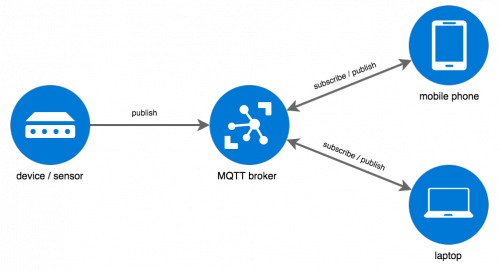
\includegraphics[width=0.9\textwidth]{MQTT.png}
	\caption[MQTT Architecture]{MQTT Architecture with the broker in the middle as a mediator between the clients~\cite{1Sheeld2018Pure-javascript-MQTT-broker.2018}.}
	\label{MQTT}
\end{figure}

A commonly used message broker is RabbitMQ which supports AMQP 0.x natively and MQTT via a plugin~\cite{RabittMQ-Documentation2018Which2018}.

AMQP needs to be distinguished between version 0.x and 1.0, as the underlying messaging paradigm has been completely revised. While for 0.x strict publishing/subscription messaging is required, version 1.0 is based on a peer-to-peer connection where a broker is not required, although possible. Due to the more sophisticated version of AMQP 1.0, fewer implementations exist.~\cite{Dizdarevic2019AIntegration}

\subsubsection{REST}
REST is an architectural paradigm describing how distributed systems can communicate with each other. It consists of five mandatory- and one optional restriction/s. If any of the five mandatory restrictions is violated, an architecture cannot be RESTful. The restrictions are client–server architecture, statelessness, cacheability, layered system, uniform interface and code on demand (optional). Roy Fielding developed REST alongside HTTP/1.1 and although it is not dependent on it, HTTP/1.1 is the primarily used protocol to implement REST. Thus, many web pages fulfill these restrictions naturally. REST messages are usually human-readable JSON files. Unlike MQTT or AMQP 0.x, REST does not rely on a broker.~\cite{Fielding2000ArchitecturalArchitectures}

\subsubsection{gRPC}
\label{sec:grpc}
For many cases in the past, it was hard for maintainers to adhere to all REST principles due to its strict nature. Moreover, REST is usually implemented with HTTP/1.1. In 2015, HTTP/2 was released to address the flaws of its predecessor~\cite{Sayfan2018REST2018}. Among those are the lack of ability of constant data streaming and latency issues.

gRPC, a remote procedure call technology introduced by Google in 2016, entirely takes advantage of HTTP/2 and thus has some advantages over REST: it allows multiplexing, binary (i.e., quick) data transfer and more. The technology behind gRPC is a remote procedure call, letting the user call remote methods as if they were local, albeit the remote method can be processed on a different hardware or system. gRPC uses protofiles to describe interface semantics. In protofiles, the user specificies service- and method names as well as message types and input/output values. Out of these protofiles, stubs can be generated which are placeholder classes for gRPC clients and servers. Unlike in most implementations of REST, gRPC does not use textual transport data like JSON but relies on Protobuf (short for protocol buffer), a binary buffer~\cite{Google-Cloud-Documentation2018Cloud2018}. For backwards compatibility towards older clients, there is a gateway available which provides transcoding from HTTP/JSON to gRPC. See figure~\ref{ESP} for the concept behind it~\cite{gRPC-Gateway-Documentation2017Grpc-gateway.2018}.

\begin{figure}[ht]
	\centering
  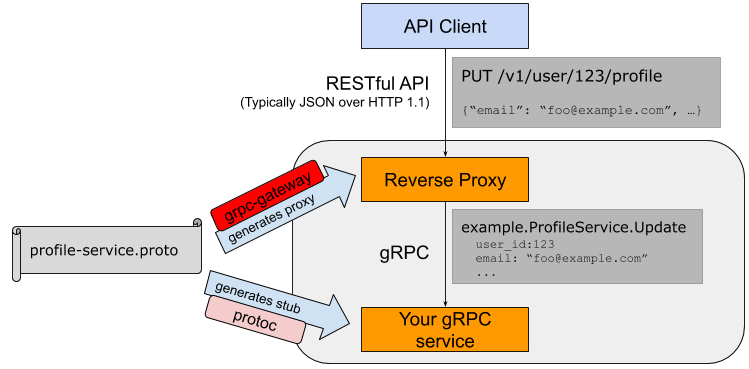
\includegraphics[width=\textwidth]{img/grpc_gateway.png}
	\caption[gRPC gateway concept]{gRPC gateway concept~\cite{gRPC-Gateway-Documentation2017Grpc-gateway.2018}. Based on a protofile, it generates a reverse proxy which handles RESTful API client requests and maps them to gRPC methods.}
	\label{ESP}
\end{figure}

The gateway is a plugin of protoc (short for protocol compiler) as part of gRPC's ecosystem. Based on a given proto file, the gRPC-gateway generates a reverse proxy offering a RESTful interface which internally maps REST/HTTP1.1 to gRPC calls. The mapping between gRPC and HTTP is described here with an example protofile directly quoted from Google's API documentation~\cite{Google-API-Documentation2019Http.proto.2019}:\\

\begin{lstlisting}[language=protobuf3,style=protobuf]
     service Messaging {
       rpc GetMessage(GetMessageRequest) returns (Message) {
         option (google.api.http) = {
             get: "/v1/{name=messages/*}"
         };
       }
     }
     message GetMessageRequest {
       string name = 1; // Mapped to URL path.
     }
     message Message {
       string text = 1; // The resource content.
     }
\end{lstlisting}

The option in the protofile enables HTTP REST to gRPC mapping:

    \begin{tabular}{c|c}
        \textbf{HTTP} & \textbf{gRPC} \\ \hline
        GET /v1/messages/123456 & GetMessage(name: "messages/123456")
    \end{tabular}

\subsubsection{GraphQL}
GraphQL is a data query and manipulation language. It was developed by Facebook and is open-source since 2015. Compared to REST, it has a more flexible and efficient approach. The increase in efficiency over REST is based on faster mobile data access, and more flexibility for the application programming interface (API) to let clients access precisely the data they need, i.e., the server modifies the data with respect to the clients' needs instead of providing one rigid resource. REST allows the user to pass a single set of arguments - the query parameters and URL segments. In GraphQL, every field and nested object can get its own set of arguments. It also lets the user pass arguments in scalar fields allowing for data transformations. An example query directly quoted from GraphQ's documentation is depicted here~\cite{GraphQL-Documentation2018Basics2018}:

\begin{lstlisting}
 {
  human(id: "1000") {
    name
    height(unit: FOOT)
  }
}
\end{lstlisting}

The corresponding response from the server is:

\begin{minipage}{\linewidth}
\begin{lstlisting}
 {
  "data": {
    "human": {
      "name": "Luke Skywalker",
      "height": 5.6430448
    }
  }
}
\end{lstlisting}
\end{minipage}

\subsubsection{OPC UA}
OPC UA is a \textit{machine-to-machine} (M2M) protocol specialized in vendor independent communication between heterogeneous machines. Until 2018, there were two means of data exchange available for OPC UA: binary data over transmission control protocol (TCP) or extended markup language (XML) data over \textit{Simple Object Access Protocol} (SOAP). Due to the higher performance, the former is primarily used nowadays.~\cite{Schleipen2016OPCVariability} 

In 2018, the OPC Foundation introduced part 14 of the OPC UA specification stack, OPC UA Publish/Subscribe~\cite{OPC-Foundation2018OPC1.04}. It is used to communicate messages between different system components without these components having to know each other’s identity. Now it is possible to use more protocols for data exchange: AMQP, MQTT, OPC UA user datagram protocol (UDP) and OPC UA Ethernet. OPC UA UDP can perform multicasts, i.e., one entity can send data to a group with the same effort as sending to a single entity. Multicasts are more performant than brokers, although do not enable time decoupling of services~\cite{Eckhardt2018AnCases}. OPC UA Ethernet is a simple Ethernet based protocol not relying on IP or UDP~\cite{OPC-Foundation2018OPC1.04}. As for the payload of the protocols, JSON or UADP are allowed. UADP is specialized for cyclic communication between, e.g., PLCs. The payload is included directly in the transport protocol.

Eckhardt et. al. performed an evaluation based on expert estimates in 2018 on how the different combinations of data exchange in OPC UA suit for the specific needs at the field, control, human-machine-interface (HMI) and enterprise level~\cite{Eckhardt2018AnCases}. See figure~\ref{fig:opc_ua_dataexchange} for an overview for the evaluated combinations.

\begin{figure}[ht]
    \centering
    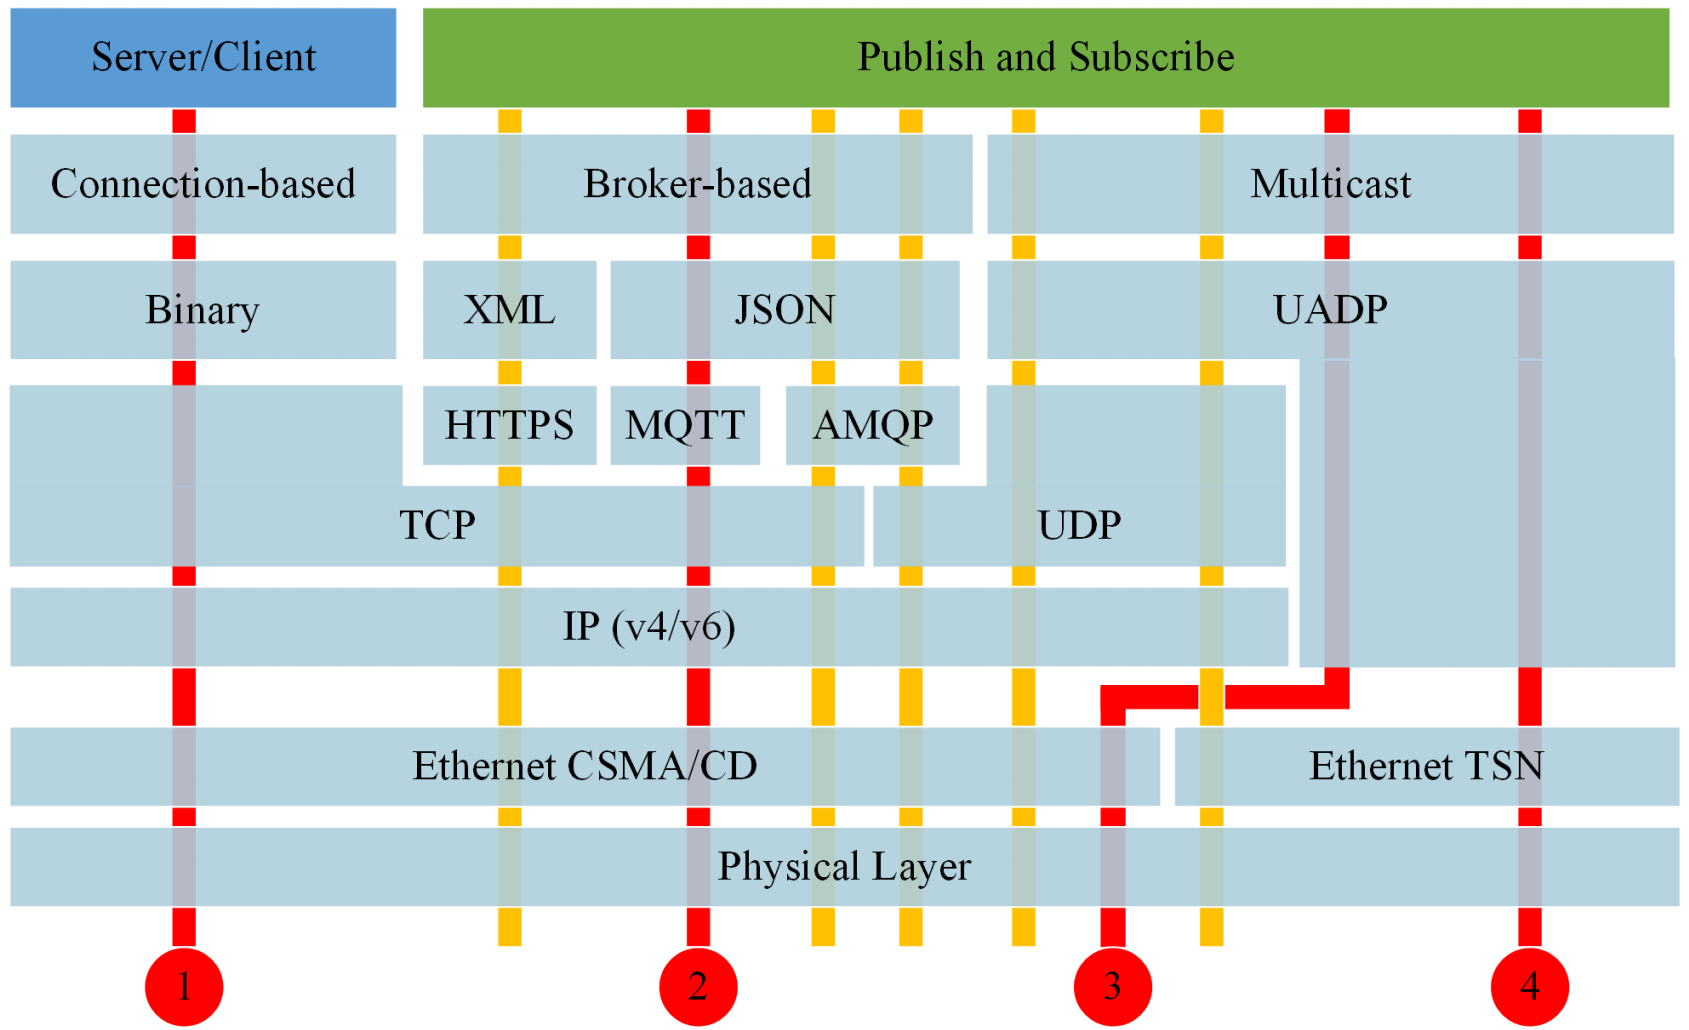
\includegraphics[width=\textwidth]{img/OPC_UA_Data_Exchange.png}
    \caption[OPC UA Data Exchange Variants]{OPC UA data exchange variants. The red and yellow vertical lines are possible variants, the red lines are evaluated in detail in~\cite{Eckhardt2018AnCases}.}
    \label{fig:opc_ua_dataexchange}
\end{figure}

The experts estimated that all combinations are suitable for HMI and enterprise level, but only combinations 3 and 4 are suited for control and field level. Combination 4 uses OPC Ethernet TSN which is OPC UA's approach of eliminating the need for fieldbus protocols~\cite{Wilmes2019ZauberwortKonvergenz}. TSN resides on OSI reference model layer 2 as a set of standards\footnote{mainly IEEE 802.1Q~\cite{2018IEEENetworks}. See~\cite{Bruckner2019AnSystems} for a full list and detailed description.} to boost ethernet networks with low latency and high availability. So-called \textbf{convergent} networks can be implemented with TSN, meaning different components (sensors, PLCs, etc.) can each arrange data streams - from synchronous low-latency to event-based. Streams can be extended or altered at any time. The main components of TSN are time synchronization enabling real-time functionalities, and scheduling and traffic shaping enabling coexistence for multiple streaming classes. \\
In practice, there are some network adapters and switches available which implement a subset of the TSN standards. The open-source automation development lab which is also responsible for the open-source project open62541\footnote{An implementation of OPC UA under the Mozilla public license 2.0 as opposed to the dual license model (i.e., proprietary for members, general public license 2.0 for non-members) of the OPC Foundation~\cite{Emde2019DieLizenzen}.} currently evaluates performance and prices of the released hardware~\cite{Emde2019DieLizenzen}. While a user currently has to accept a price increase of 1000-2000\,\% as opposed to conventional hardware, the tests confirm TSN to be as performant as established fieldbus systems~\cite{Emde2019DieLizenzen}.

There was also an attempt to create an OPC UA to REST adapter by Ronnhölm in 2018~\cite{Ronnholm2018IntegrationThesis}. Although OPC UA allows HTTP on the application layer, there is an incentive: OPC UA is not RESTful. RESTful HTTP is centered around resources that can be identified by a URL and a message. Any body of data may therefore be manipulated independently of any intermediary application logic. This is not the case with HTTP in OPC UA. Ronnhölm claims (\cite{Ronnholm2018IntegrationThesis},~page 26): \say{To enable exchange with OPC UA servers without the use of an OPC UA stack, a holistic translation must translate both structural and foundational aspects of OPC UA. This means that translation must bypass OPC UA transport protocols, secure channel management, serialization and OPC UA services - all in a way that avoids semantic dependencies and preserves translation transparency.} He concludes that a subset of OPC UA services can be transformed to REST when combined with standard create-request-update-delete methods.

\subsection {Deployment Options}
\label{deploymentoptions}
In the last decades, most software applications had a monolithic character which did not focus much on scalability and agile development. With the progress in digitalization, applications had to become more flexible and faster. To address the challenge of deploying applications highly automated, container architectures came about. Unlike virtual machines which need an operating system, runtime and system variables to operate well, Docker and other virtualization technologies are sandbox systems which can imply all the mentioned features and furthermore can run on almost any operating system. In the following, two possible virtualization technologies are briefly introduced, namely Heroku and Docker. They are motivated by pointing out how they are superior to virtual machines in the context of microservices.~\cite{Wurbs2017Docker2018.}

Docker is an open-source standard for operating-system-level virtualization. If Docker is installed on an operating system, it is possible to run several applications on the machine simultaneously, with low start and stop times and little overhead. These applications can rely on different platforms, dependencies, runtimes, etc. The technology behind it is a daemon which shares low-level components with the host operating system. A hypervisor is not necessary (see figure~\ref{container} for an illustration). 

\begin{figure}[ht]
	\centering
  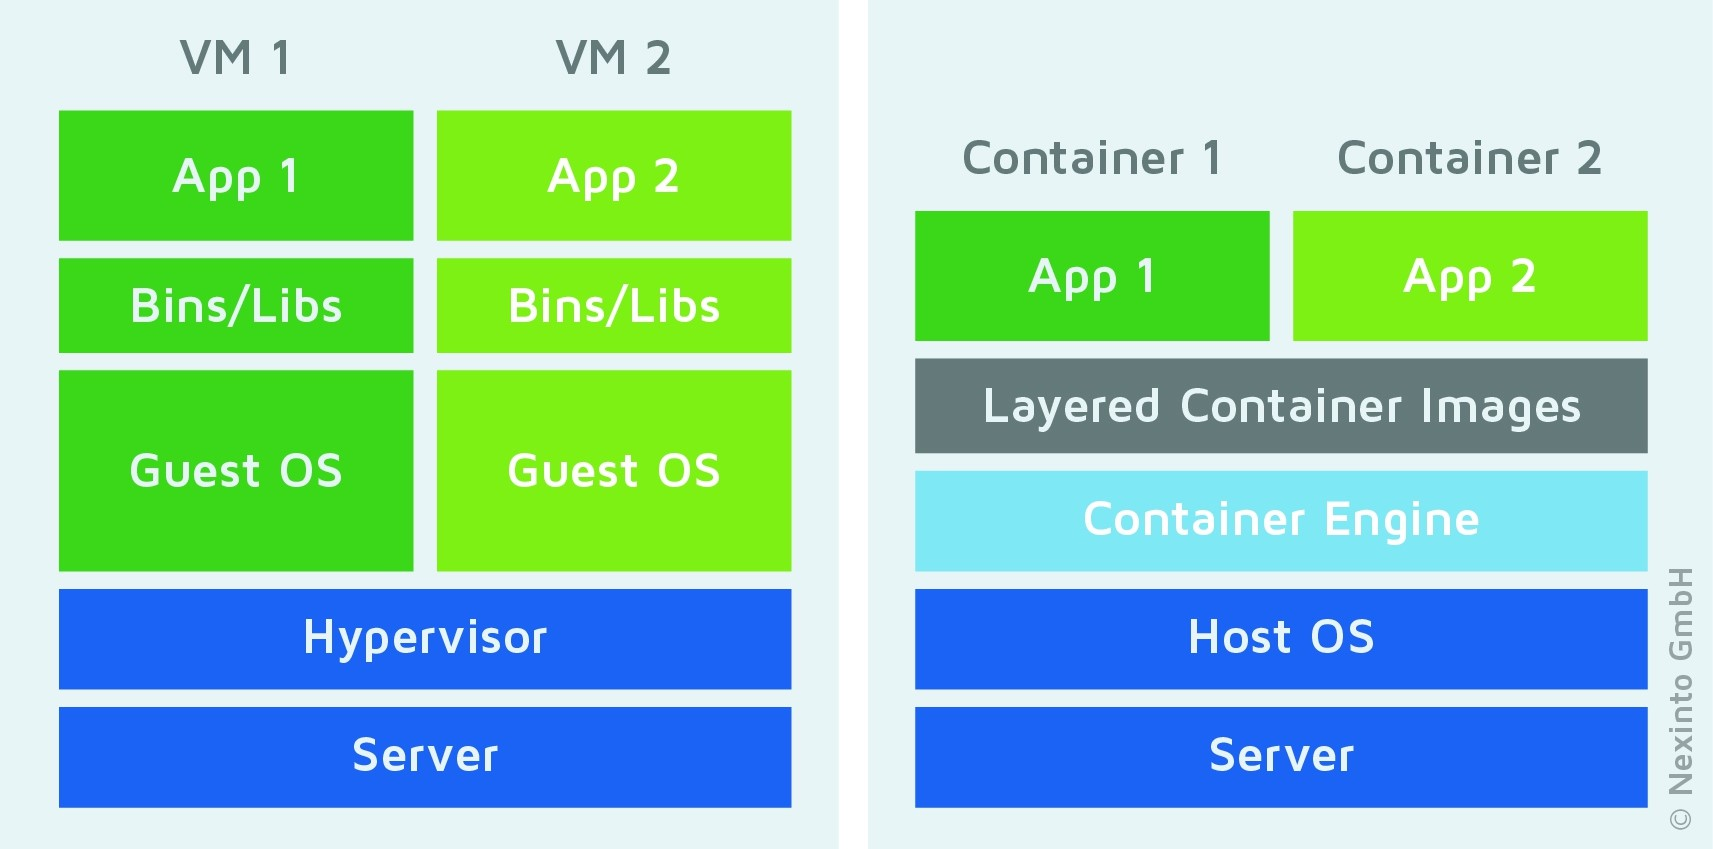
\includegraphics[width=0.7\textwidth]{containervsvm.jpg}
	\caption[Docker vs Virtual Machine Architecture]{Virtual machine architecture on the left versus container architecture on the right. Docker does not rely on a hypervisor.~\cite{Wurbs2017Docker2018.}}
	\label{container}
\end{figure}

To virtualize applications, Docker uses containers which are built up on Docker images. Images are read-only templates that are built from a set of instructions written in a dockerfile. They offer one great advantage - a layered file system. This enables the user to easily add or update applications very quickly. Images can be shared in a public/private registry called Docker Hub. \\
Last but not least, development and operations of applications can be harmonized through a combination of Docker and a continuous integration and continuous delivery platform. 

Heroku is a platform as a service provider whose underlying technology shares some core concepts with Docker. E.g., BuildPacks are a set of scripts which are used to set up the final state of an image. The pendant on the Docker side is called dockerfile (see Thurig's blog~\cite{Thurig2014Docker2018} for a full description of the similarities and table~\ref{dockerandheroku} for a list of pendants). However, there are also differences between the two alternatives. The main one is the dependency on the Heroku platform on the Heroku side, whereby on the Docker side one is completely flexible in choosing any environment from Raspberry Pi to cloud platform providers like Amazon Web Services. The latter also means a surplus of workload on infrastructure on the Docker side. Also, one is less flexible on the prices. Heroku has a staged price model ranging from 0 to 500\,\$ per month and dyno. Docker is again more flexible in letting one just paying for the hosting and storaging and leaving the additional features provided by Heroku aside.~\cite{Chris2017Why2018} 


\begin{table}
\begin{center}
      \caption[Similar core concepts of Docker and Heroku]{Similar core concepts of Docker and Heroku. \cite{Thurig2014Docker2018}}
  \begin{tabular}{ l | l }
    Docker & Heroku  \\ \hline
Dockerfile &	BuildPack \\ 
Image	& Slug\\ 
Container&	Dyno\\ 
Index	&Add-Ons\\ 
CLI	&CLI
  \end{tabular}
  \label{dockerandheroku}
\end{center}
\end{table}

\section{Object Detection Service Interface Semantic}
If two humans want to communicate with one another, they need matching channels and need to speak the same language. A channel is a mean of transport for information, e.g., sign language, smoke signs and mobile phones. If one entity tries to call someone via phone if the other does not have a phone or the caller enters the wrong number and the other has its cellphone turned off, they cannot communicate. In case they both have a phone, the called entity answers and both speak a common language (e.g., English), the exchange of information can be achieved. Communication within technical systems faces the same challenges. As for the right channel, models like the open systems interconnection (OSI) basic reference model for information technology standardized by the international organization for standardization (ISO) layer the transfer of information. It ranges from the physical layer consisting of peaks in currents and voltages up until the application layer which includes direct user interaction, resource availability and so forth~\cite{InternationalOrganizationForStandardization1996ISO/IECEd.}. This model and the protocols adhering to it ensure that information is delivered safely between communicating entities. However, this model does not imply the semantics of the payload or the language, as stated in the analogy above. 

This section introduces two possible ways of how an ODS service interface semantic can be designed. One resides in the IT and cloud domain whereas the other rather resides in the OT domain.

\subsection{Google Cloud Vision API}
Google Cloud Vision (GCV) API offers a publicly available REST and gRPC interface~\cite{Google-Cloud-Documentation2019Google2019-04-26}. OD operations can be executed on the cloud. The upside of this approach is excessive computing power and an attractive pay-per-use price model. The downside is the limitation of the configurability of Google's ODs and the lacking transparency of where and how the data is stored and evaluated. An example gRPC call for annotating images with labels of objects is depicted here:

\begin{lstlisting}[language=protobuf3,style=protobuf]
    rpc AsyncBatchAnnotateFiles(AsyncBatchAnnotateFilesRequest) returns (Operation)
\end{lstlisting}


\subsection{OPC UA Vision}
A currently proposed semantic standard for OD processes is \textbf{OPC UA Vision}. It includes a finite state machine abstracting an industrial system from its diverse conditions and transitions. Moreover, it offers an information model covering the administration of recipes, configurations and results. With the help of the state machine, it is defined which information of the information model is retrievable. The content of the three administration objects remains proprietary with the advantage of covering a broad range of OD scenarios.

\subsubsection{State Machine}
According to the specification, powering up and shutting down a vision system are mandatory processes and thus should be handled in a standardized manner. Also, the handling of errors should be the same for all vision systems. The design of the core operation state, however, shall remain with the manufacturer. Automatic mode as a sub-state of operational mode is one proposed way of designing it. The state machine for a typical vision system in automatic mode is depicted in figure~\ref{fig:OPCStateMachineAutomatic}. An example of this operation would be a PLC guiding an inspection system for position determination. When powered on, the system enters the preoperational state through loading a configuration marked as active. From there, an operation mode is either automatically chosen by the system or manually triggered. An operation mode is any sub-state machine of the operational state. The automatic mode is chosen and enters the initial state. Then a recipe can be prepared, describing properties, procedures and parameters for a machine vision job. The recipe may include information for a single and/or continuous execution. A single execution would be e.g. determining the pose of an object; a continuous execution could be monitoring and surveillance systems which constantly process and acquire data. When the system is done with an execution or execution step, e.g., taking a picture from one of four angles, it sends results asynchronously to the client. If the system is shut down, it should be put into halt mode first where a safe power-off is assured. From all states, it is possible to enter the error state. Errors are handled aligning with their severity and sometimes need acknowledgment or confirmation by a human before the system can be reset to preoperational state.

\begin{figure}[ht]
    \centering
    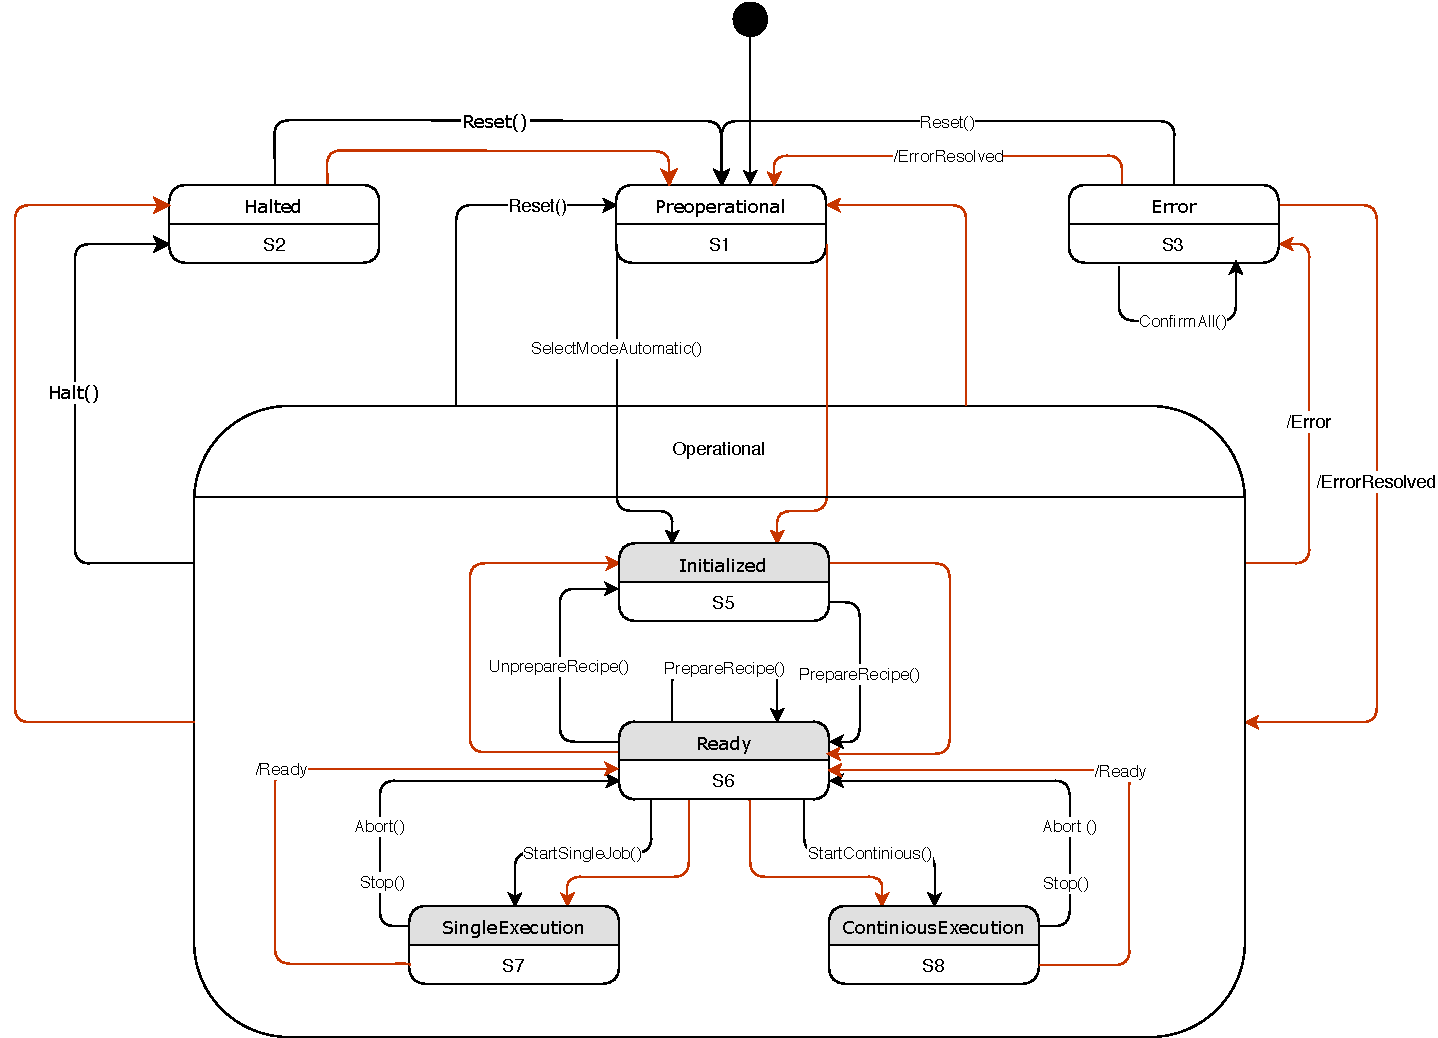
\includegraphics[width=\textwidth]{img/OPCUAVisionVisionAutomaticModeStateMachineStates.pdf}
    \caption[OPC UA Vision state machine in automatic operation mode]{OPC UA Vision state machine in automatic operation mode. Red Lines indicate automatic transitions induced by the vision system with optional effects prefixed with a slash. Black lines indicate method induced transitions with the method name as the trigger. The black circle is the entry point of the state machine. All of the states can have optional sub-state machines. States marked in grey are substates.~\cite{VDMA2018OPC40100-1:2018-11}}
    \label{fig:OPCStateMachineAutomatic}
\end{figure}

\subsection{Information Model}
The information model formally describes all datasets, types, methods, address- and namespaces. See figure~\ref{fig:OPCInfoModelOverview} for an overview and figure~\ref{fig:OPCInfoModelNotation} for an explanation of the notation. Configuration, recipes and result are the three types that have to be dealt with when using OPC UA Vision.

\say{Even identical vision systems may vary in some details. In order to produce the same results the vision systems have to be adjusted individually e.g., calibrated. Within this document, the set of all parameters that are needed to get the system working is called a configuration. Configurations can be used to align different vision systems that have the same capabilities, so that these systems produce the same results for the same recipes. The ConfigurationManagement handles all configurations that are exposed by the system. Only one configuration can be active at a time. This active configuration affects all recipes used in the machine vision system.}~(\cite{OPC-Foundation2018OPC1.04}, chapter~7.2)

\say{Properties, procedures and parameters that describe a machine vision task for the vision system are stored in a recipe. Usually there are multiple usable recipes on a vision system. This specification provides methods for activating, loading, and saving recipes. Recipes are handled as binary objects. The interpretation of a recipe is not part of this specification. Recipes are potentially complex entities. A recipe may contain (possibly nested) references to sub-recipes and it may be used for several products. The internal composition of recipes – including the referencing of sub-recipes – is outside the scope of this specification.}~(\cite{OPC-Foundation2018OPC1.04}, appendix~1.2.1 and~1.2.2) For an example recipe life cycle, see appendix~\ref{chap:recipelifecycle}.

\say{ResultManagementType provides methods to query the results generated by the underlying vision system. Results can be stored in a local result store.}~(\cite{OPC-Foundation2018OPC1.04}, chapter~7.8)

XML nodesets can be used to import information models to an OPC UA server. A screenshot of an example information model uploaded to an OPC UA demo server and viewed by UAExpert is depicted in~\ref{fig:uaexpert}. It also shows how methods are called, in this example a simple product of two numbers. An important, more sophisticated method of the OPC UA Vision specification is StartSingleJob (subpart of StateMachineType, not depicted in the information model overview in~\ref{fig:OPCInfoModelOverview}). Usually it is called by a PLC to trigger a machine vision task. Its signature consists of following parameters:

\begin{minipage}{\linewidth}
\begin{tabbing}
    space \= space \= spacespacespace \= spacespacespacespace \= spacespacespace \kill
    \>  StartSingleJob(\\
    \>  \>  (in)	 \> 	String          \> MeasId\\
    \>  \>  (in)	 \> 	String          \> PartId\\
    \>  \>  (in)	 \> 	RecipeIdType    \> RecipeId\\
    \>  \>  (in)	 \> 	ProductIdType   \> ProductId\\
    \>  \>  (out)	 \> 	String          \> JobId\\
    \>  \>  (out)	 \> 	Int32           \> Error); 
\end{tabbing}
\end{minipage}

In another section of the specification, the data types are defined, e.g. RecipeIdType, which is a structure including an Id, a version and a hash.

When the method is called, it triggers transition from state Ready to SingleExecution in the state machine as depicted in~\ref{fig:OPCStateMachineAutomatic}.

\begin{figure}[ht]
    \centering
    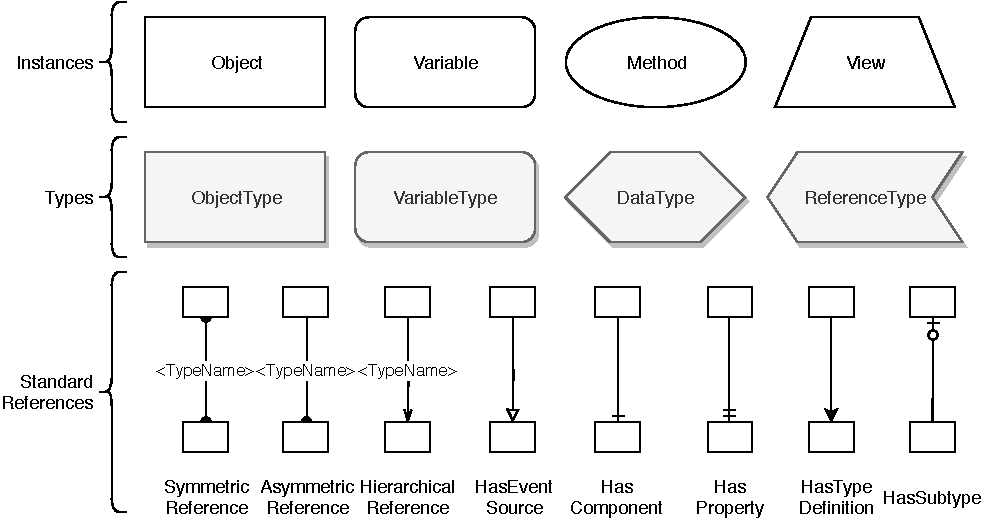
\includegraphics[width=0.8\textwidth]{img/OPCUAVisionInformationModelNotation.pdf}
    \caption[OPC UA Vision Information Model Notation]{OPC UA Vision Information Model Notation.\cite{VDMA2018OPC40100-1:2018-11}}
    \label{fig:OPCInfoModelNotation}
\end{figure}

\begin{figure}
    \centering
    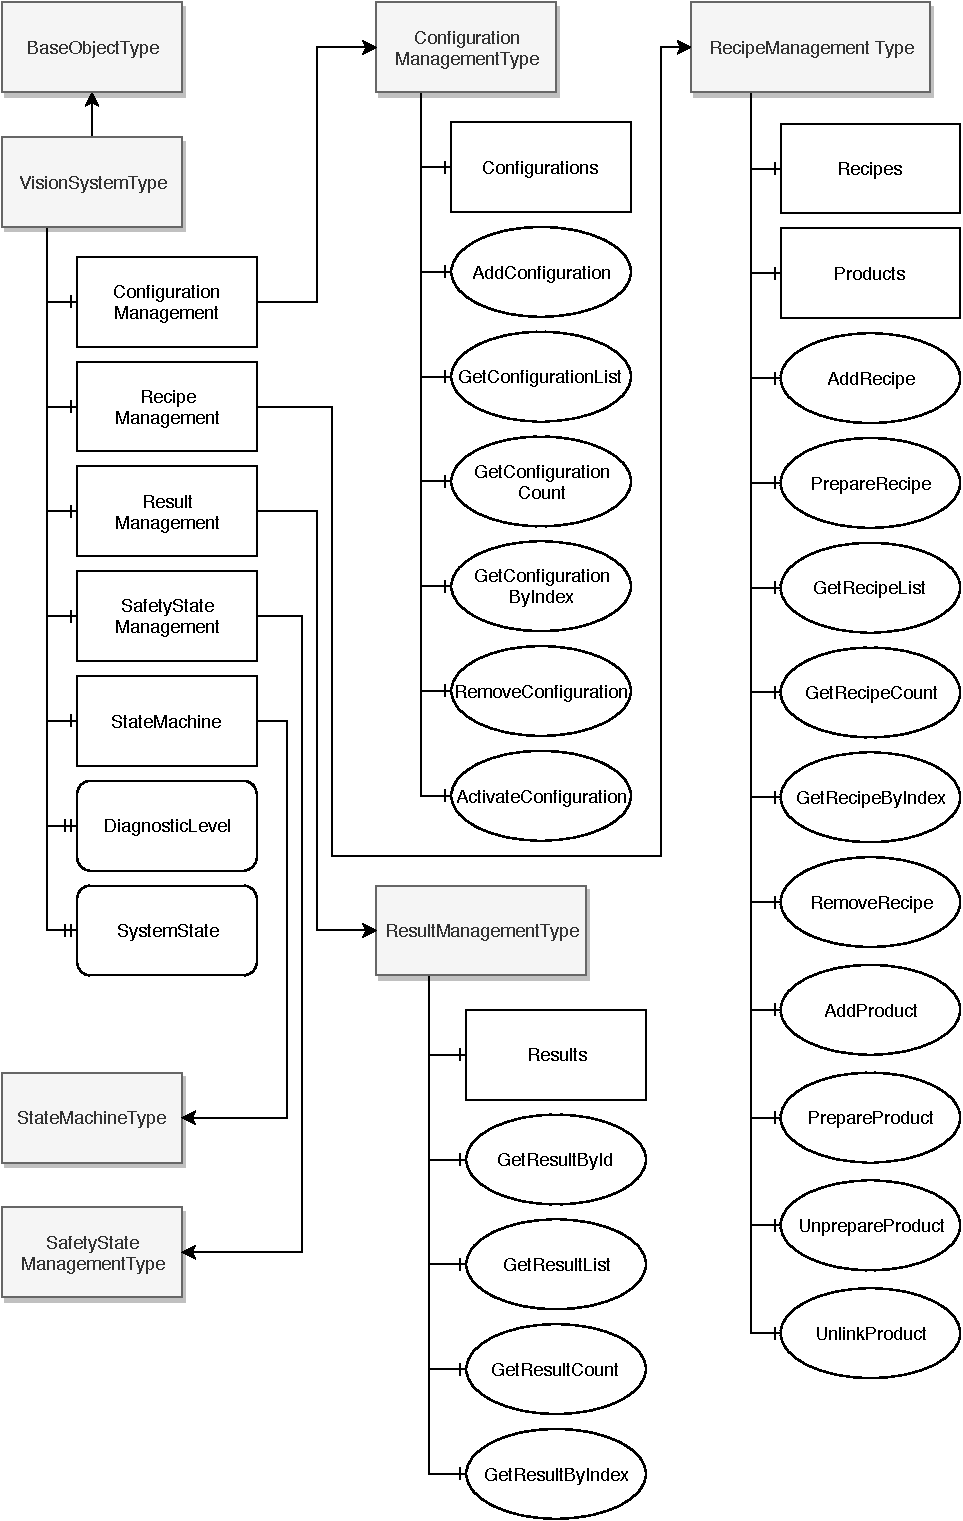
\includegraphics[height=0.9\textheight]{img/OPCUAVisionInformationModelOverview.pdf}
    \caption[OPC UA Vision Information Model Overview]{OPC UA Vision Information Model Overview. See fig. \ref{fig:OPCInfoModelNotation} for a description of the notation.~\cite{VDMA2018OPC40100-1:2018-11}}
    \label{fig:OPCInfoModelOverview}
\end{figure}

\begin{landscape}
\begin{figure}[ht]
    \centering
    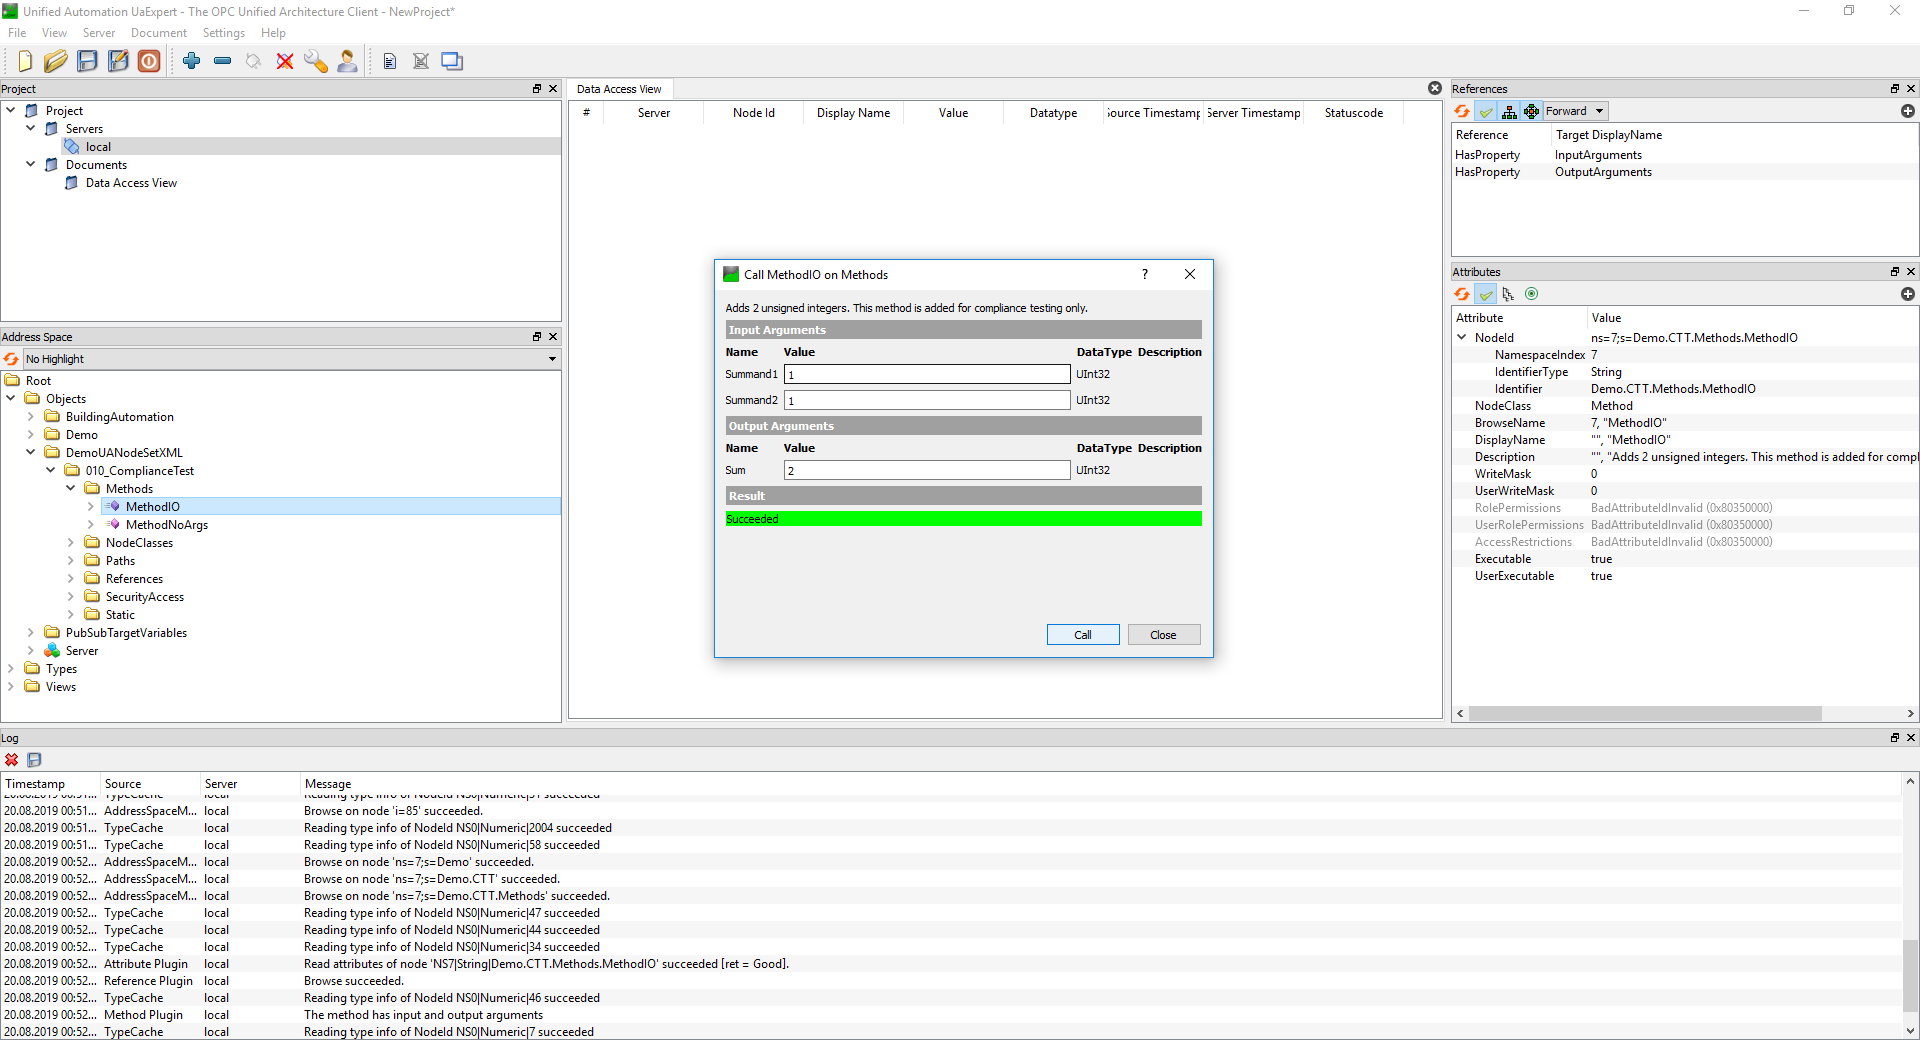
\includegraphics[width=1.5\textwidth]{img/UAExpertScreenshot.png}
    \caption[Example Information Model in UAExpert]{Screenshot of UAExpert showing an example information model in the folder hierarchy on the left. The data access view in the middle is a list of nodes and their corresponding current values. Also, a simple method call multiplying two values is depicted on the bottom right corner. The multiply method implies references and attribute which are pointed out on the right.}
    \label{fig:uaexpert}
\end{figure}
\end{landscape}

\section{Summary}
The most important aspects of the state of the art sections are:
\begin{itemize}
    \item Contemporary ODM use 3D and RGB-D images for pose determination in \textbf{two phases}.
    \item Service interface protocols have to be chosen appropriately for every application.
    \item Containerization is a convenient way of deploying services.
    \item OPC UA Vision is based on an information model and a state machine based on which is decided which information is retrievable.
    \item Recipes are vendor-specific.
\end{itemize}
